%-------------------------------------------------------------------------------
%	NAME:	report.tex
%	AUTHOR: Connor Beardsmore - 15504319
%	LAST MOD:	01/05/17
%	PURPOSE:	FCC Assignment Report
%	REQUIRES:	NONE
%-------------------------------------------------------------------------------

\documentclass[]{article}
\usepackage[ margin=3cm ]{geometry}
\usepackage{graphicx}
\usepackage{fancyhdr}
\usepackage{float}
\usepackage{hyperref}
\usepackage{transparent}
\usepackage{multicol}
\usepackage{amsmath}
\usepackage[final]{pdfpages}
\usepackage{listings}
\usepackage{color}
\usepackage{algorithmicx}
\usepackage{algpseudocode}
\usepackage{amssymb}
\usepackage[style=chicago-authordate,backend=biber]{biblatex}

\pagestyle{fancy}
\fancyhf{}
\lhead{Connor Beardsmore - 15504319}
\rhead{FCC200}
\lfoot{May 2017}
\rfoot{\thepage}

\pagenumbering{arabic}
\graphicspath{{./images/}}

\addbibresource{bib/references.bib}
\nocite{*}

%-------------------------------------------------------------------------------
% CODE HIGHLIGHTING FOR LISTINGS
\definecolor{codegreen}{rgb}{0,0.6,0}
\definecolor{codegray}{rgb}{0.5,0.5,0.5}
\definecolor{codepurple}{rgb}{0.58,0,0.82}
\definecolor{backcolour}{rgb}{0.99,0.99,0.99}

\lstdefinestyle{mystyle}{
	backgroundcolor=\color{backcolour},   
	commentstyle=\color{codegreen},
	keywordstyle=\color{magenta},
	numberstyle=\tiny\color{codegray},
	stringstyle=\color{codepurple},
	basicstyle=\footnotesize,
	breakatwhitespace=false,         
	breaklines=true,                 
	captionpos=b,                    
	keepspaces=true,                 
	numbers=left,                    
	numbersep=5pt,                  
	showspaces=false,                
	showstringspaces=false,
	showtabs=false,                  
	tabsize=2
}

\lstset{style=mystyle}


%-------------------------------------------------------------------------------
\begin{document}
%-------------------------------------------------------------------------------
% TITLE PAGE

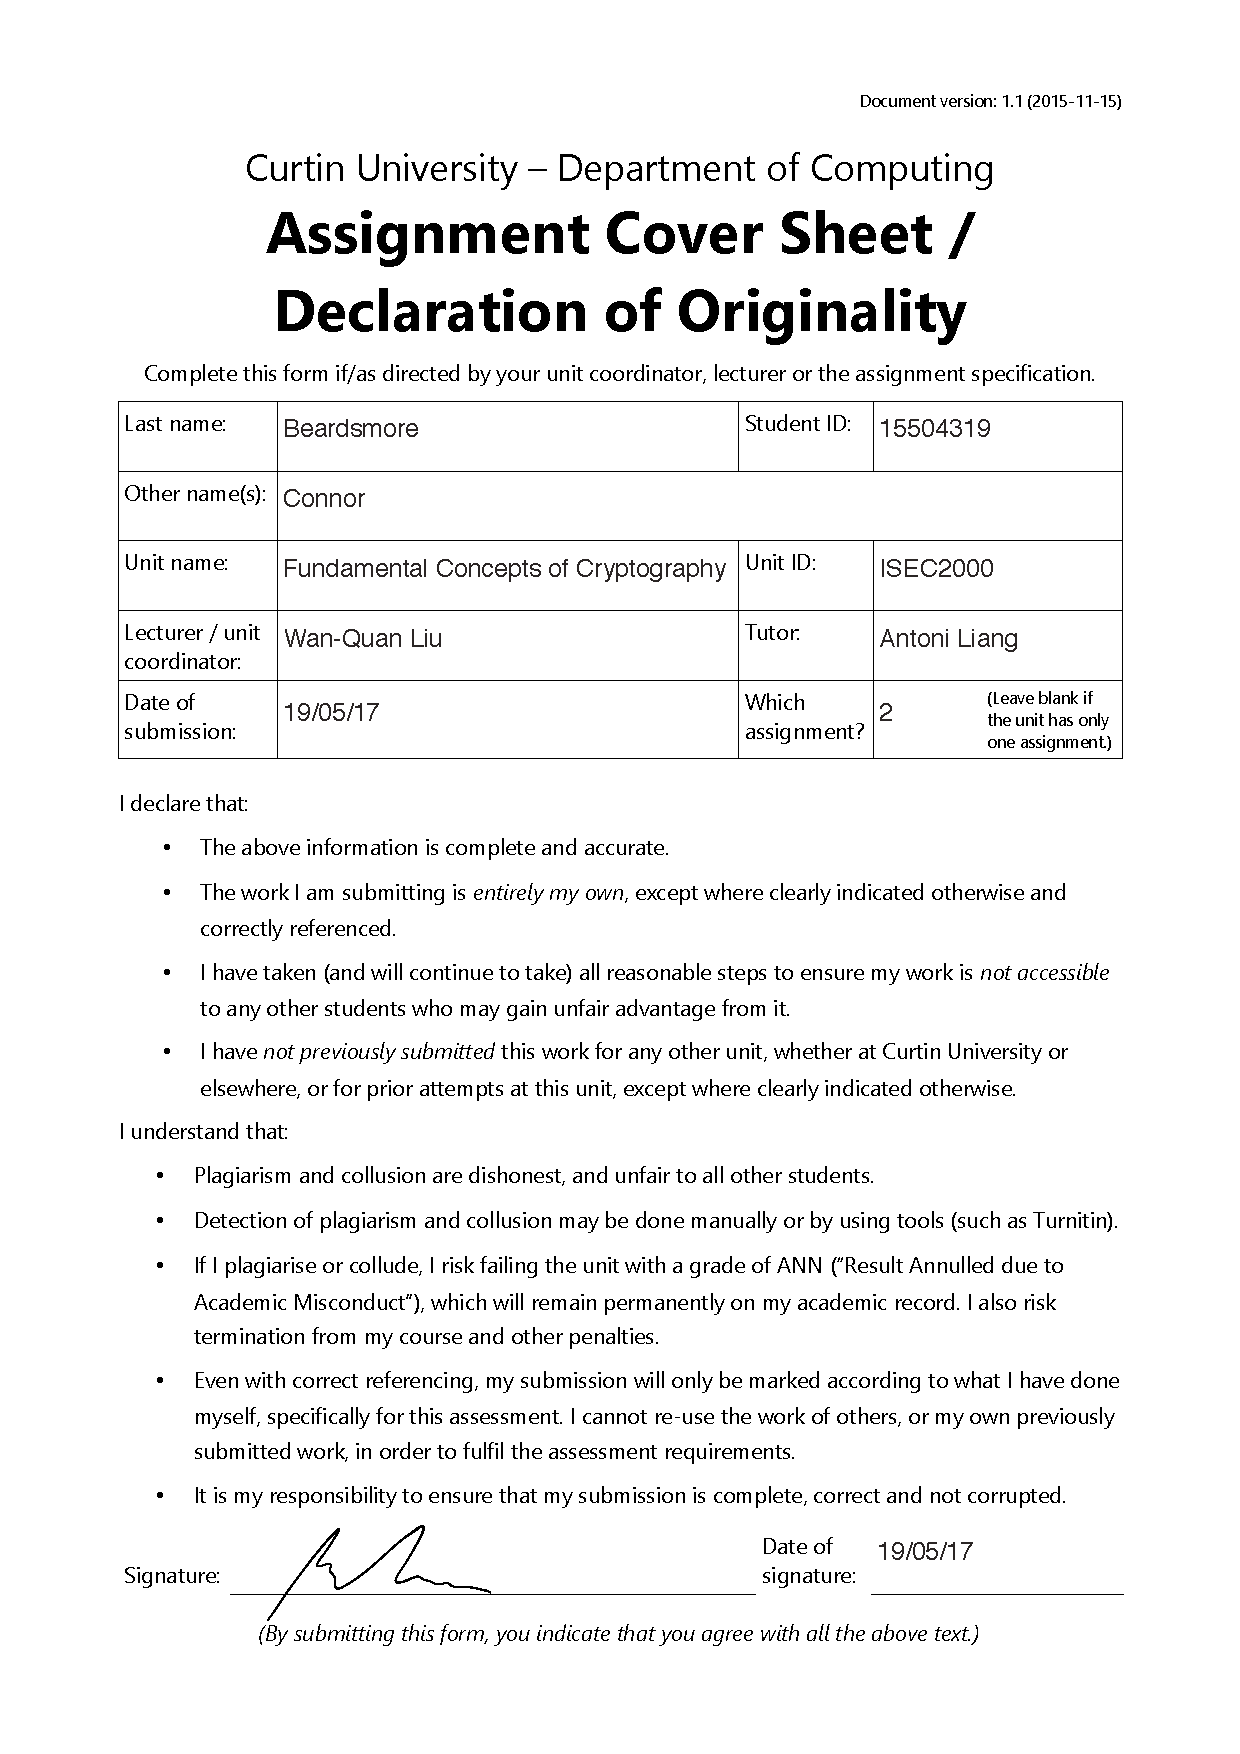
\includepdf[]{./images/cover_page.pdf}

\begin{titlepage}
	\begin{center}
		\vspace*{1cm}
		\LARGE\textbf{FCC200 Report}
		\break
		RSA Cryptosystem Implementation
		\vspace{1cm}
		\break
		\Large\textbf{Connor Beardsmore - 15504319} 
		\vspace{15cm}

		\normalsize
		Curtin University \\
		Science and Engineering \\
		Perth, Australia \\
	    May 2017
	    
	\end{center}
\end{titlepage}

%-------------------------------------------------------------------------------
% BINARY MODULAR EXPONENTIATION
\vspace*{-0.8cm}
\section*{\hfil RSA Implementation\hfil}

\subsection*{Modular Exponentiation}
\noindent
Modular exponentiation is used to calculate the remainder when a base \textit{b} is raised to an exponent \textit{e} and reduced by some modulus \textit{m}. The simple right-to-left method provided by \cite{alttext} utilizes exponentiation by squaring. The full Java code for the implementation of this method is illustrated below. The running time of this algorithm is $O(log\;e)$ which is a huge improvement over more simplistic methods of time $O(e)$ (\cite{maintext}).

\vspace{0.5cm}
\lstinputlisting[language=C,linerange={58-92} ]{../../rsa/numberTheory.c}{}

\noindent
The code above was utilized to calculate the following example:

$$236^{239721}\;mod\;2491=236$$

\pagebreak

%-------------------------------------------------------------------------------
% RSA IMPLEMENTATION
\vspace*{-0.8cm}

\subsection*{RSA Testing}

\begin{figure}[H]
	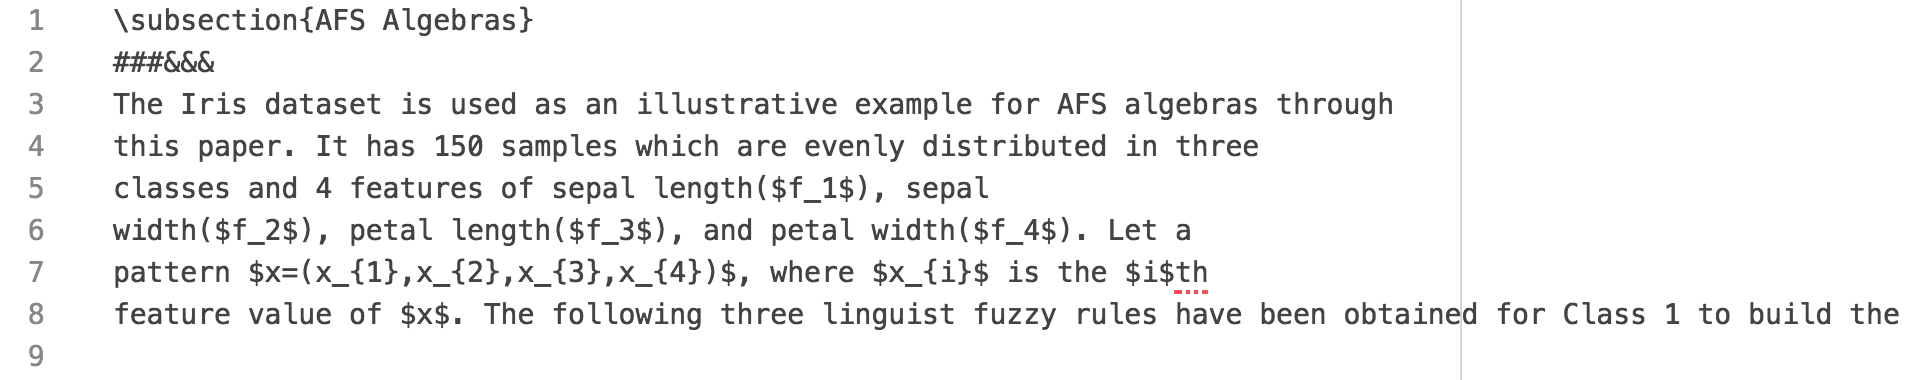
\includegraphics[height=\textheight/6,width=\textwidth]{rsa_plain1.png}
	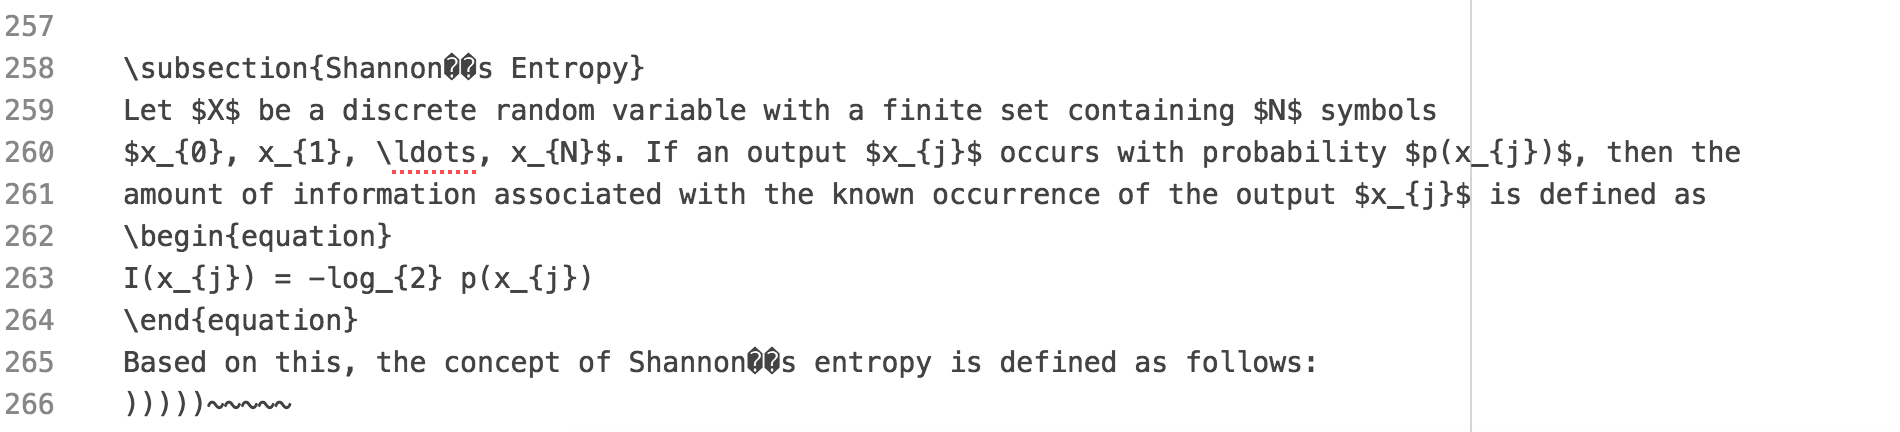
\includegraphics[height=\textheight/6,width=\textwidth]{rsa_plain2.png}	
	\caption{RSA Plaintext}
	\centering
\end{figure}

\begin{figure}[H]
	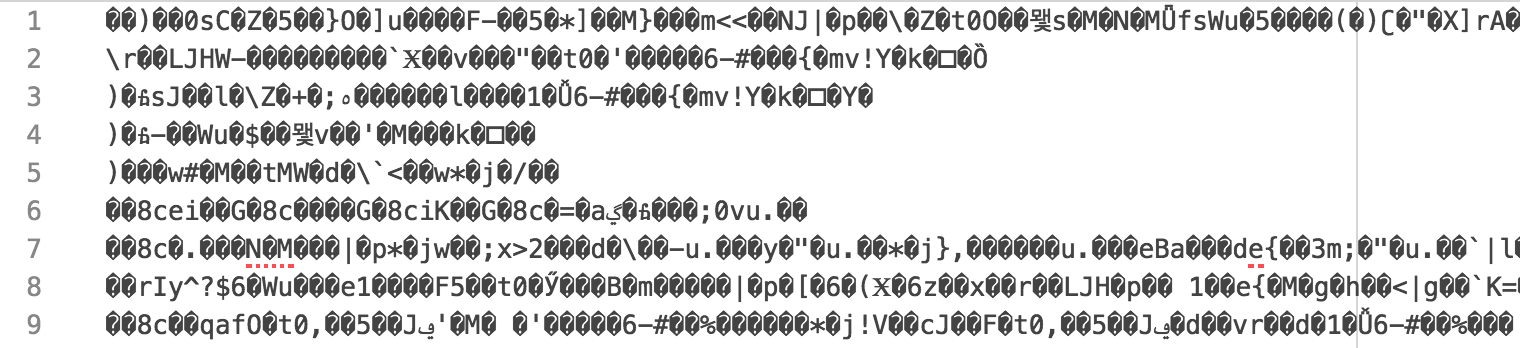
\includegraphics[width=\textwidth]{rsa_cipher1.png}
	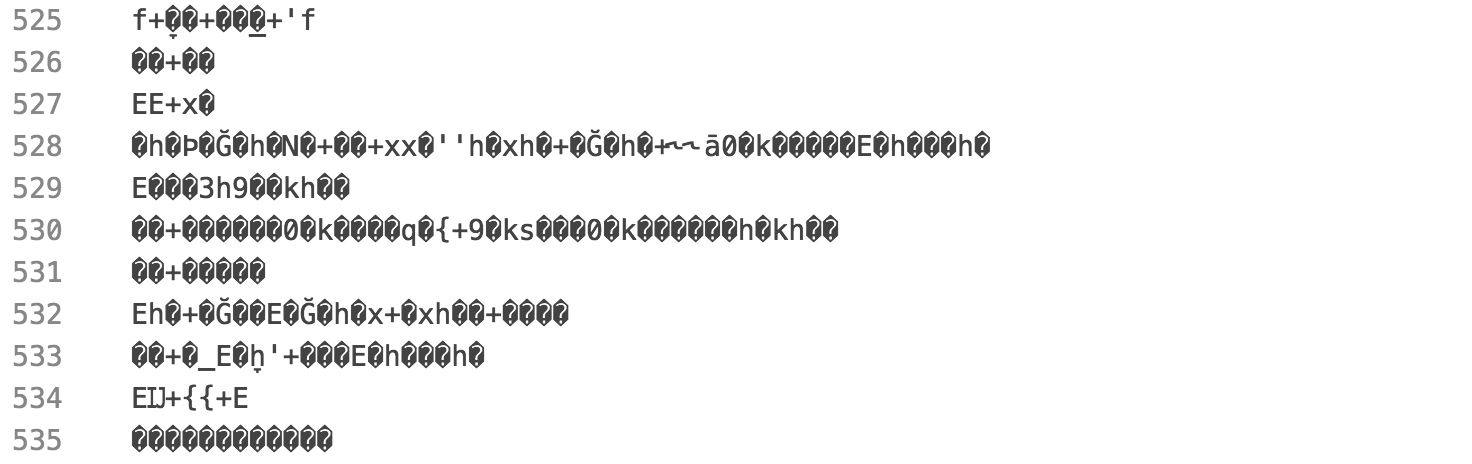
\includegraphics[width=\textwidth]{rsa_cipher2.png}	
	\caption{RSA Ciphertext}
	\centering
\end{figure}

\begin{figure}[H]
	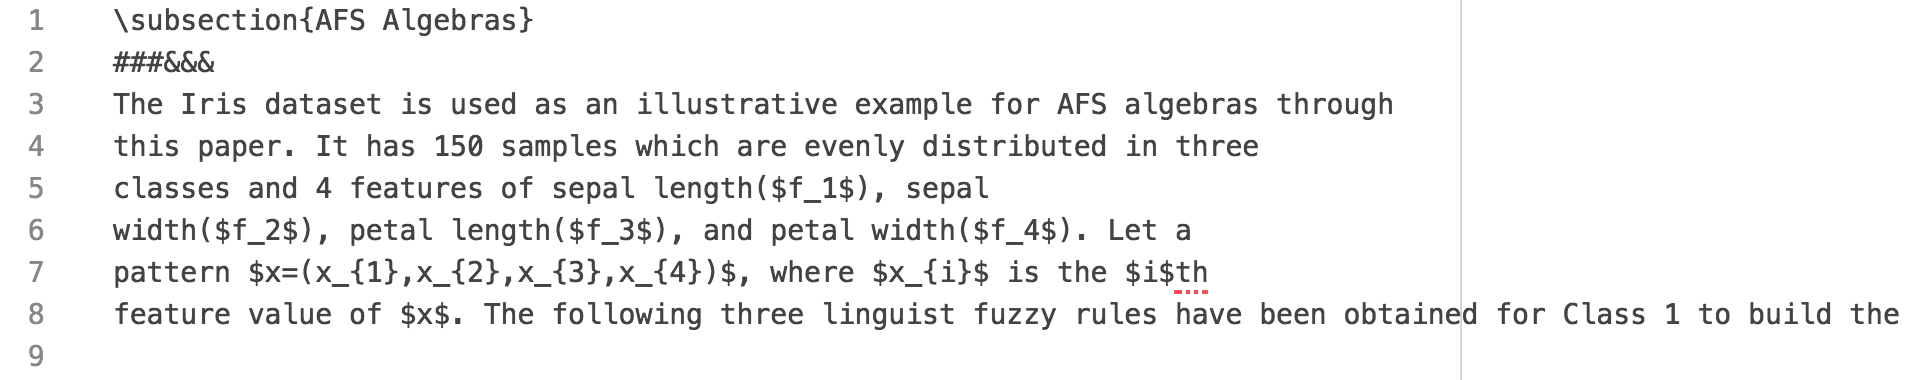
\includegraphics[height=\textheight/6,width=\textwidth]{rsa_plain1.png}
	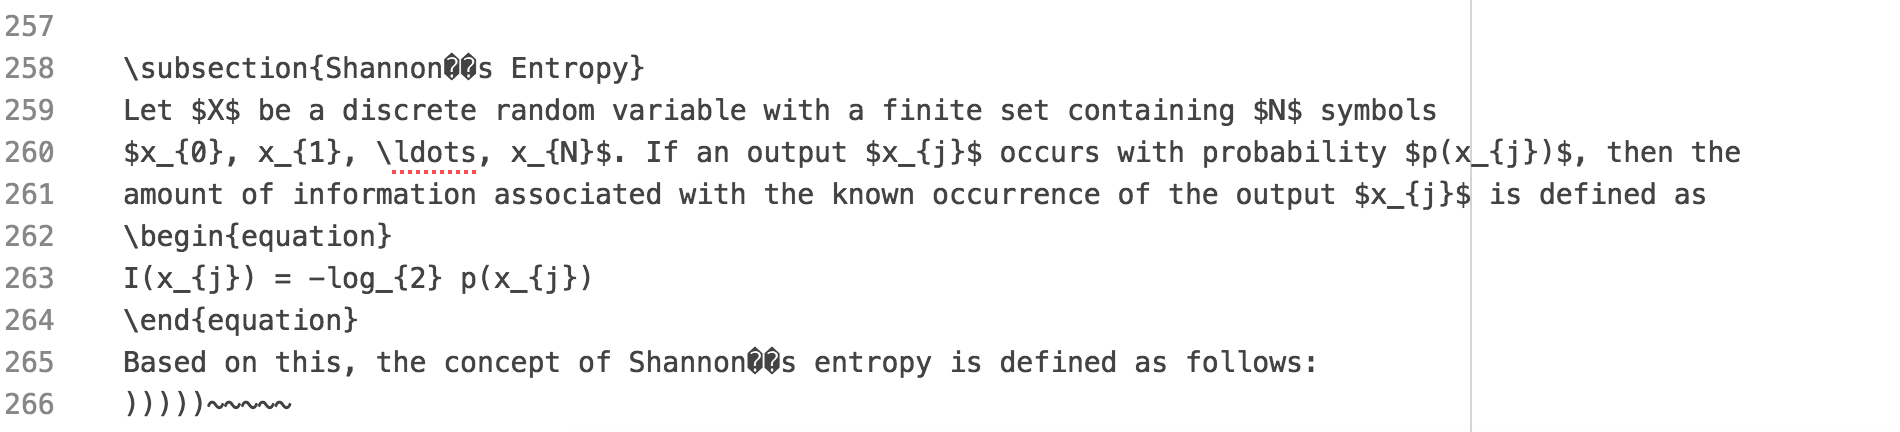
\includegraphics[height=\textheight/6,width=\textwidth]{rsa_plain2.png}	
	\caption{RSA Recovered Plaintext}
	\centering
\end{figure}

\pagebreak

%-------------------------------------------------------------------------------
% ADDITIONAL QUESTIONS

\vspace*{-0.8cm}
\section*{\hfil Additional Questions\hfil}

\subsection*{Signature Forgery}

 If a receiving person were to try to verify message m′, they would input H(m′) along with the previously mentioned variables into the verification function and find that the output is equal to r. This would lead the receiver to believe that m′ originated from Alice. This situation, however is not as worrying as it would appear as it would be very unlikely that m′ contained any meaningful information. This is very similar to the Birthday Problem mentioned in Lecture 8, while it is quite probable to find two people in a group of thirty or more who share a birthday, but it is far less probable to find somebody whose birthday matches a specific birthday. It may be trivial for Bob to craft an m′ with a hash matching H(m′), it is far less likely for Bob to craft a meaningful message with a hash matching H(m′).

\subsection*{Birthday Attack}

\vspace{0.5cm}
\begin{center}
\textit{In a group of 23 randomly selected people, the probability that two\\ of them share the same birthday is larger than 50\%}
\end{center}
\vspace{0.5cm}

\noindent
Firstly, the probability that two people have different birthdays is found:

$$1-\frac{1}{365}=\frac{364}{365}=0.99726$$

\vspace{0.5cm}
\noindent
This can be extended to determine if three people have different birthdays:

$$1-\frac{2}{365}=\frac{363}{365}=0.99452$$

\vspace{0.5cm}
\noindent
Utilizing conditional probability (\cite{lecture2}) we can construct the probability that all 23 people have different birthdays. This is simply represented as a series of fractions with their product producing the resultant probability:

$$1\times(1-\frac{1}{365})(1-\frac{2}{365})...(1-\frac{22}{365})=0.493$$

\vspace{0.5cm}
\noindent
To find the probability that two of the people have the same birthday, we inverse this number by subtracting from the total probability (1):

$$1-0.493=0.507=50.7\%$$

\vspace{0.5cm}
\noindent
It is thus evident that the probability of two people in a set of 23 random selected shared the same birthday is greater than 50\%.

\pagebreak

%-------------------------------------------------------------------------------
% RSA CODE

\vspace*{-0.8cm}
\begin{center}
	\section*{RSA Source Code}
\end{center}

\subsection*{makefile}
\lstinputlisting[language=make,linerange={} ]{../../rsa/Makefile}\pagebreak{}
\subsection*{numberTheory.h}
\lstinputlisting[language=C,linerange={} ]{../../rsa/numberTheory.h}\pagebreak{}
\subsection*{numberTheory.c}
\lstinputlisting[language=C,linerange={} ]{../../rsa/numberTheory.c}\pagebreak{}
\subsection*{main.h}
\lstinputlisting[language=C,linerange={} ]{../../rsa/main.h}\pagebreak{}
\subsection*{main.c}
\lstinputlisting[language=C,linerange={} ]{../../rsa/main.c}\pagebreak{}

%-------------------------------------------------------------------------------   
% REFERENCES

\break
\setlength\bibitemsep{4\itemsep}
\printbibliography[title={References}]

%-------------------------------------------------------------------------------
\end{document}   
%-------------------------------------------------------------------------------: